\documentclass[12pt]{article}
\usepackage{amsmath}
\usepackage{fullpage}
\usepackage[authoryear,round]{natbib}
\usepackage{lineno}
\usepackage{graphicx} 
\usepackage{setspace}
\doublespacing

\title{Density-dependent selection and the limits of relative fitness}
\author{Jason Bertram $^{1,\ast}$ \\ 
Joanna Masel $^{1}$}

\date{}

\begin{document}

\maketitle

\noindent{}1. Department of Ecology and Evolutionary Biology, University of Arizona, Tucson, AZ 85721.

\noindent{}$\ast$ Corresponding author; e-mail: jbertram@email.arizona.edu.

\bigskip

\textit{Keywords}: Lottery model, competitive Lotka-Volterra, $r$/$K$-selection, interference competition, eco-evo.

\bigskip

\textit{Author contributions}: JB and JM conceptualized the manuscript. JB did the formal analysis. JB wrote the manuscript with review and editing from JM. 

\bigskip

\textit{Running title}: Density-dependence and relative fitness

\bigskip

\textit{Acknowledgments}: We thank Peter Chesson and Joachim Hermisson for many constructive comments on an earlier and quite different version of this manuscript. This work was financially supported by the National Science Foundation (DEB-1348262) and the John Templeton Foundation (60814).

\linenumbers{}
\modulolinenumbers[1]

\newpage{}


\section*{\centering \huge  Density-dependent selection and the limits of relative fitness}

\bigskip

\subsection*{Abstract}

Selection is commonly described in terms of relative fitness. Yet when selection is strong, the ecological view of selection in density-regulated populations seems to be incompatible with widely-used, constant-density relative fitness models such as the Wright-Fisher. Here we analyze the population ecological limits of relative fitness using a novel generalization of the Wright-Fisher model in which population density depends dynamically on the demographic rates of the types present. Our model contains a ``reproductive excess’’, and clearly distinguishes between density-dependent selection and selection-dependent density. These two effects are confounded in standard models of density-regulated population growth. Both effects are necessary, in combination with strong selection, for relative fitness to break down in populations close to demographic equilibrium. Remarkably, both effects are not sufficient: we give an example of strong selection on a density-regulating trait subject to density-dependent selection that conforms to the relative fitness description almost exactly. We reiterate the importance of reproductive excesses in many species, which allows even strong selection to have no effect on density. Our model also offers a possible alternative to relative fitness when the latter is untenable, as is likely the case far from demographic equilibrium. 

\noindent (191 words)



\newpage{}


\section*{Introduction}

There are a variety of different measures of fitness. Some widely used examples in evolutionary ecology are expected lifetime reproductive ratio $R_0$, intrinsic population growth rate $r$, saturation population density (often labeled ``$K$'') \citep{benton_2000}, and invasion fitness \citep{metz_1992}. In addition, ``relative fitness'' is the standard in much of evolutionary biology, particularly evolutionary genetics, where attention is generally restricted to relative genotypic proportions \cite[pp. 468]{barton_2007}. The variety of fitness measures is not problematic in itself, because different measures may be more useful in different circumstances. But it should be clear how the measure being used is connected to the processes of birth and death which govern population biology \citep{metcalf_2007,doebeli_2017}. While such a connection is fairly clear for absolute fitness measures like $r$, relative fitness seems largely divorced from population biology. It has even been proposed that relative fitness be justified from measure theory, abandoning population biology altogether \citep{wagner_2010}. Given the ubiquitous use of relative fitness, it is important that we understand its population ecological basis, both to clarify its domain of applicability, and as part of the broader challenge of synthesizing ecology and evolution.

Constant relative fitness values can be justified as a linear approximation \cite[pp. 277]{ewens_2004} \citep[Chap. 4]{charlesworth_1994} which is close to exact provided that selection is sufficiently weak and stable over time. Yet strong, temporally-variable selection occurs widely in nature and the lab, including in wild \textit{Drosophila}, where population density varies by orders of magnitude each seasonal cycle \citep{messer_2016,bergland_14}. The question is whether relative fitness can be used when selection is not vanishingly weak. In general, age-structured populations that reproduce by outcrossing do not permit strong selection to be represented in terms of type-specific relative-fitness constants \citep[Chap. 4]{charlesworth_1994}. We will therefore restrict our attention to asexual haploids with little or no age structure, where it is easier to evaluate how the success or failure of the relative fitness description is tied to the underlying population ecological assumptions. 

The basis of relative fitness is straightforward in the absence of crowding: it simply represents differences in intrinsic population growth rate. In discrete time, the change in frequency of type $i$ is $\Delta p_i=\left(\frac{W_i}{\overline{W}}-1\right) p_i$, where $W_i$ is the intrinsic absolute growth factor of type $i$, and $\overline{W}=\sum_i W_i p_i$ is the population mean $W$. Here we can rescale $W$ however we please and replace it with ``relative fitness'' $w$ without affecting the ratio $\frac{W_i}{\overline{W}}=\frac{w_i}{\overline{w}}$. In continuous time, the canonical selection equation is $\frac{d p_i}{dt}=(r_i-\overline{r}) p_i$, where $W$ is replaced by the intrinsic exponential growth rate $r$ \citep[pp. 26]{crow_1970}. If there are two types present, a wildtype and a mutant for instance, then the continuous time canonical selection equation can be written as
\begin{equation}
\frac{d p_i}{dt}=s p_i(1-p_i), \label{eq:canonical}
\end{equation}
where the constant selection coefficient $s$ is the difference in $r$ between types. The corresponding adaptive sweeps follow a logistic curve. 

The difficulty with Eq.~\eqref{eq:canonical} arises in crowded populations. Since crowded and uncrowded conditions are so different, we expect that $s$ will often depend on density \citep{travis_2013}. Eq.~\eqref{eq:canonical} is then no longer a complete description of selection --- we would also need to specify a model for how density is changing. Note that frequency-dependent selection does not raise similar problems; Eq.~\eqref{eq:canonical} is still a complete description of selection even if its behavior is more complicated due to $s$ depending on frequency. Population genetics traditionally evades the issue of density-dependent selection by simply assuming that total population density $N$ has reached its equilibrium value, which is assumed to be a fixed constant. The selection coefficient $s$ now abstractly parameterizes the rate at which selection changes relative frequencies, and no longer corresponds to differences in intrinsic growth rates $r$. 

However, MacArthur famously argued that when population growth is density-regulated, selection in crowded populations is intimately connected to the ability to keep growing at higher densities than other types can tolerate \citep{macarthur_1967}. The classic example is the logistic model, where the type with the greatest saturation population density ``$K$'' excludes the others (Fig.~\ref{fig:Ksel}a). Similarly, the ``$R^*$ rule'', a central tenet of resource competition theory, states that when growth is limited by a single homogeneous consumable resource, the type able to deplete the resource to the lowest equilibrium density $R^*$ excludes the others \citep{grover_1997}. Differences in $R^*$ will often entail differences in saturation density. The Lotka-Volterra competition model also couples selection in crowded populations to density except in special cases \citep{smouse_1976,mallet_2012}. In these examples, both $N$ and $s$ change during, and as a result of, adaptive sweeps. It would therefore seem that the ubiquitous constant-$N$, relative fitness description of selection is incompatible with a huge class of population ecological processes driving selection (Fig.~\ref{fig:Ksel}b), even in the absence of age-structure and mating.

\begin{figure}
\centering
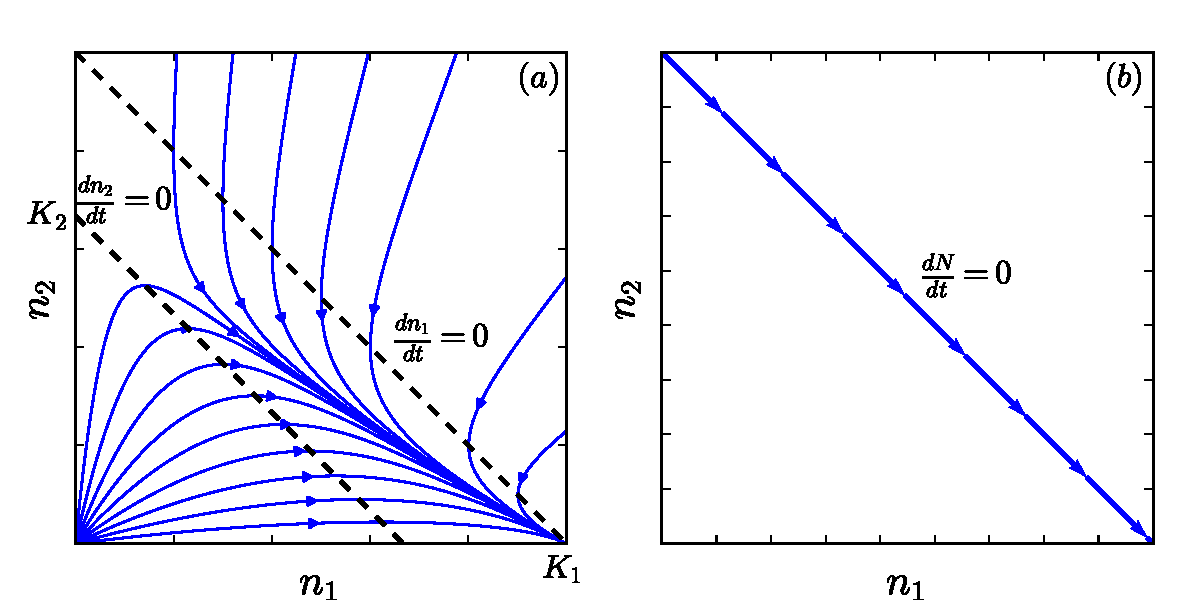
\includegraphics[scale=0.8]{Kplot.pdf}
\caption{\label{fig:Ksel} Selection in crowded environments shown as a phase diagram for the densities of two types $n_1$ and $n_2$. (a) The logistic model $\frac{dn_1}{dt}=r_1(1-\frac{n_1+n_2}{K_1})n_1$ and $\frac{dn_2}{dt}=r_2(1-\frac{n_1+n_2}{K_2})n_1$ with $r_1=r_2$ and $K_1>K_2$. (b) The constant-$N$, relative fitness description of selection.}
\end{figure}

In light of this difficulty, the relative fitness description has been justified in broadly two different ways for crowded populations (we do not discuss Wagner's [\citeyear{wagner_2010}] measure-theoretical justification, which is independent of population biology). The first is to simply assume that selection is density-independent but relax the assumption of constant $N$ by allowing density to change as a result of selective sweeps \citep[pp. 468]{barton_2007} \citep{prout_1980}. Obviously this does not address the problem that $s$ can, in reality, depend on density. Type-specific responses to density are at the center of MacArthur's argument and the density-dependent selection literature that grew out of it (e.g. \citep{roughgarden_1979}). 

The second justification, which primarily grew out of a controversy over Haldane's ``cost of selection'', is to appeal to the existence of a ``reproductive excess'' of juveniles that are more fragile than their adult counterparts \citep{turner1968population,kimura1969natural,nei1971fertility}. Selection can then be concentrated at the juvenile phase, uncoupling selection from population density at the adult phase unless it is so strong that the reproductive excess is depleted. This justifies Eq.~\eqref{eq:canonical} because, for a population in demographic equilibrium, selective sweeps do not affect density, and so the density-dependence of selection does not matter. Unfortunately this reproductive excess literature is also poorly integrated with population ecology. \cite{kimura1969natural} took constant $N$ as a requirement and then derived some variants of the logistic model that satisfy this requirement. \cite{nei1971fertility} proposed a model with an explicit representation of reproductive excess, but used an unusual model of competition based on pair-wise interactions which was only defined for at most two different types. As a result, the role of reproductive excesses in justifying Eq.~\eqref{eq:canonical} is still largely verbal.

Here we study the population ecology of relative fitness using a novel model of density-dependent population growth based on territorial contests. Rather than attempting to make sense of relative fitness in existing standard models of population growth (e.g. \citep{kimura1969natural,mallet_2012}), we instead do the reverse, and attempt to make population ecological sense of the widely-used Wright-Fisher relative-fitness model. Our starting point is the classic lottery model of territorial contest \citep{sale_77,chesson_1981}. Like the Wright-Fisher model, the classic lottery assumes a saturated population with constant $N$, and fitness involves a product of fertility and juvenile viability \citep[pp. 185]{crow_1970}, but unlike the Wright-Fisher model, generations can overlap. Our first task is to generalize the lottery model to create a variable-density version of the Wright-Fisher model with overlapping generations (sections ``Model'' and ``Analytical approximation of the variable-density lottery''). 

Equipped with this new model, we turn to the evaluation of Eq.~\eqref{eq:canonical}. We first discuss selection on the ability to contest territories, which behaves like a pure constant-$N$, relative fitness trait, and discuss how this fits with MacArthur's analysis of selection in crowded populations (section ``$K$-selection and selection-dependent density''). We then consider selection on density-regulating traits (section ``Density-regulating traits and the threat of strong selection''), and conclude by contrasting the classical density-dependent selection literature with our results (``Discussion'').
 
\section*{Model}\label{sec:model}

\subsection*{Assumptions and definitions} 

We assume that reproductively mature individuals (``adults'') each require their own territory to survive and reproduce. All territories are identical, and the total number of territories is $T$. Time advances in discrete iterations, each representing the time from birth to reproductive maturity. In a given iteration, the number of adults of the $i$'th type will be denoted by $n_i$, the total number of adults by $N=\sum_i n_i$, and the number of unoccupied territories by $U=T-N$. We assume that the $n_i$ are large enough that stochastic fluctuations in the $n_i$ (``drift'') can be ignored (with $T$ also assumed large to allow for small type densities $n_i/T$).

\begin{figure}
\centering
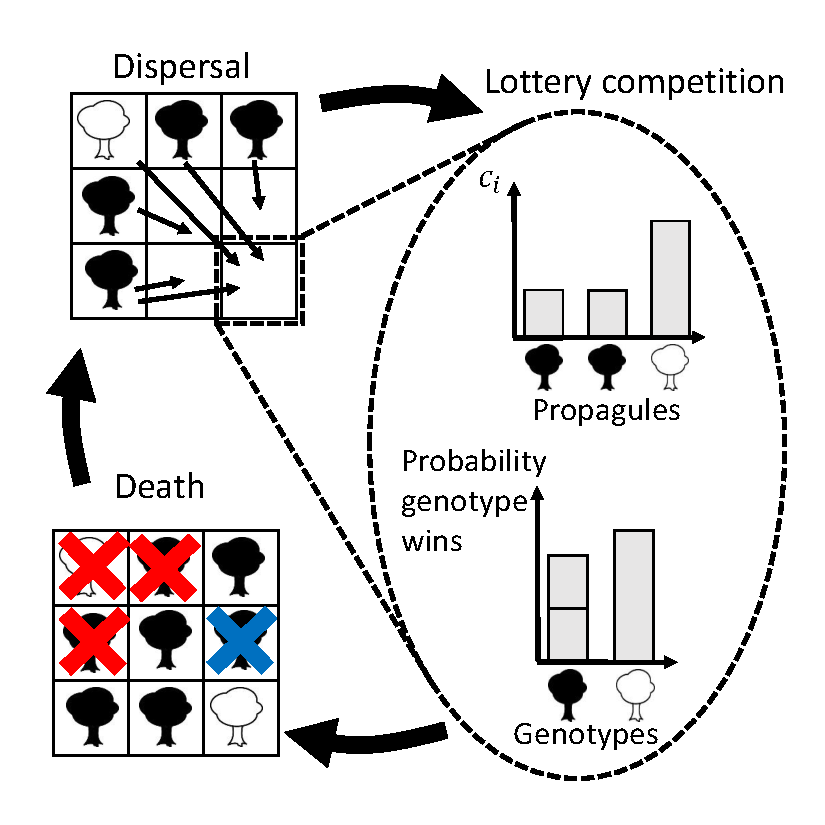
\includegraphics[scale=0.8]{lottery.pdf}
\caption{\label{fig:lottery} Each iteration of our model has three elements. First, propagules are produced by adults and dispersed at random (only propagules landing on unoccupied territories are shown). Some territories may receive zero propagules. Lottery competition then occurs in each unoccupied territory that receives a propagule (only illustrated in one territory). Each type has a probability proportional to $c_i x_i$ of securing a given territory, where $c_i$ measures competitive ability and $x_i$ is the number of propagules that disperse there. In the illustrated territory, the black type disperses more propagules but is a poorer competitor. Territories are then made available by deaths among those adults present at the start of the iteration (red crosses).}
\end{figure}

Each iteration, adults produce new offspring (``propagules''). These disperse at random, regardless of distance from their parents, and independently of each other (e.g. there is no avoidance of territories crowded with propagules). We assume that adults cannot be ousted by juveniles, so that propagules landing on occupied territories are doomed. We assume that each adult from type $i$ produces a constant number $b_i$ of successfully dispersing propagules; the number of propagules dispersing to unoccupied territories is then given by $m_i=b_in_iU/T$. The total number of these propagules will be denoted $M=\sum_i m_i$. Note that due to our assumption of uniform dispersal, the parameter $b_i$ can be thought of as a measure of ``colonization ability'', which combines fecundity and dispersal ability \citep{levins_71,tilman_94,bolker_99}. 

The number of propagules of the $i$'th type landing in any particular territory is denoted $x_i$. We assume that $x_i$ follows a Poisson distribution $p_i(x_i)=l_i^{x_i} e^{-l_i}/x_i!$, where $l_i=m_i/U$ is the mean territorial propagule density for type $i$ (the total propagule density will be denoted $L=\sum_i l_i$). This is strictly only an approximation of random dispersal, but it is an excellent approximation given our assumption that the $n_i$ are large enough that drift can be ignored (Appendix A).

When multiple propagules land on the same territory, the victor is determined by lottery competition: type $i$ wins a territory with probability $c_i x_i/\sum_j c_j x_j$, where $c_i$ is a constant representing relative competitive ability (Fig. \ref{fig:lottery}). We expect that a fraction $p_1(x_1)\ldots p_G(x_G)$ of the $U$ unoccupied territories will have the propagule composition $x_1,\ldots,x_G$. Type $i$ is expected to win a proportion $c_i x_i/\sum_j c_j x_j$ of these. Ignoring fluctuations about these two expectations (due to our no-drift, large $n_i$, large $T$ approximation), type $i$'s territorial acquisition is given by
\begin{equation}
\Delta_+ n_i=U\sum_{x_1,\ldots,x_G} \frac{c_i x_i}{\sum_j c_j x_j} p_1(x_1)\cdots p_G(x_G), \label{eq:growthsumuncoupled}
\end{equation}
where the sum only includes territories with at least one propagule present.

Finally, we assume that adult mortality only occurs in adults present at the start of the  iteration, and at a constant, type-specific per-capita rate $0\leq d_i\leq 1$. Thus, the overall change in type abundances is
\begin{equation}
\Delta n_i=\Delta_+ n_i-d_i n_i. \label{eq:delttot}
\end{equation}
Fig.~2 illustrates one iteration of the model. 

\subsection*{Connection to the Wright-Fisher and classic lottery models}

In the classic lottery model \citep{chesson_1981}, unoccupied territories are assumed to be saturated with propagules from every type $l_i\gg 1$. From the law of large numbers, the composition of propagules in each territory will then not deviate appreciably from the mean composition $l_1,l_2,\ldots,l_G$ ($G$ is the number of types present), and so the probability that type $i$ wins any particular unoccupied territory is approximately $c_i l_i/\sum_j c_j l_j$. Then the numbers of territories won by each type $\Delta_+ n_1,\Delta_+ n_2,\ldots,\Delta_+ n_G$ follow a multinomial distribution with $U$ trials and success probabilities $\frac{c_1 l_1}{\sum_j c_j l_j},\frac{c_2 l_2}{\sum_j c_j l_j},\ldots,\frac{c_G l_G}{\sum_j c_j l_j}$, respectively. Type $i$ is expected to win a proportion $c_i l_i/\sum_j c_j l_j$ of the $U$ available territories, and deviations from this expected outcome are small (since $T$ is large by assumption), giving 
\begin{equation}
\Delta_+ n_i=\frac{c_i l_i}{\sum_j c_j l_j}U=\frac{c_i l_i}{\overline{c}L}U, \label{eq:lottery}
\end{equation}
where $\overline{c}=\sum_j c_j m_j/M$ is the mean competitive ability for a randomly selected propagule. In section ``Analytical approximation of the density-dependent lottery'', we derive a generalization of Eq.~\eqref{eq:lottery} that accommodates arbitrary propagule densities $l_i$.
 
There is a close connection between the classic lottery model and the Wright-Fisher model of genetic drift \citep{svardal_2015}. In the Wright-Fisher model, type abundances are sampled each generation from a multinomial distribution with success probabilities $w_i n_i/\sum_j w_j n_j$, where $w$ is relative fitness and the $n_i$ are  type abundances in the preceding generation. Population size $N$ remains constant. This is equivalent to the classic lottery model with non-overlapping generations ($d_i=1$ for all $i$) and relative fitness given by $w_i=b_i c_i$ i.e. a product of fertility and viability \citep[pp. 185]{crow_1970}. Thus, the classic lottery model is essentially the Wright-Fisher model extended to allow overlapping generations, but ignoring drift. This means that our extension of the classic lottery model to arbitrary densities represents a variable-density generalization of the Wright-Fisher model (we also do not consider drift here).

\section*{Results}

\subsection*{Analytical approximation of the variable-density lottery}

Eq. \eqref{eq:growthsumuncoupled} involves an expectation over the time-dependent dispersal distributions $p_i$, and is thus too complicated to give intuition about the dynamics of density-dependent lottery competition. We now evaluate this expectation. 

Similarly to the high-$l_i$ approximation of the classic lottery model, we replace the $x_i$ with appropriate mean values, although we cannot simply replace $x_i$ with $l_i$ as in Eq.~\eqref{eq:lottery}. The classic lottery model breaks down for types with low propagule density ($l_i\ll 1$) because territorial acquisition is then not correctly represented by a lottery in each territory with the mean propagule density. For a type with low propagule density $l_i\ll 1$, we have $x_i=1$ in the territories where its propagules land, and so its growth comes entirely from territories which deviate appreciably from $l_i$. To account for this, we separate Eq. \eqref{eq:growthsumuncoupled} into $x_i=1$ and $x_i>1$ parts. Our more general approximation only requires that there are no large discrepancies in competitive ability (i.e. we do not have $c_i/c_j\gg 1$ for any two types). We obtain (details in Appendix B)
\begin{equation}
\Delta_+ n_i\approx \left[e^{-L}+(R_i+A_i)\frac{c_i}{\overline{c}}\right]l_i U, \label{eq:master}
\end{equation}
where
\begin{equation}
R_i=\frac{\overline{c}e^{-l_i}(1-e^{-(L-l_i)})}{c_i +\frac{\overline{c}L- c_il_i}{L-l_i}\frac{L-1+e^{-L}}{1-(1+L)e^{-L}}},\nonumber \label{eq:Dr}
\end{equation}
and
\begin{equation}
A_i=\frac{\overline{c}(1-e^{-l_i})}{\frac{1-e^{-l_i}}{1-(1+l_i)e^{-l_i}}c_il_i+\frac{\overline{c}L- c_il_i}{L-l_i}\left(L\frac{1-e^{-L}}{1-(1+L)e^{-L}}-l_i\frac{1-e^{-l_i}}{1-(1+l_i)e^{-l_i}}\right)}. \nonumber \label{eq:Da}
\end{equation}

Comparing Eq. \eqref{eq:master} to Eq. \eqref{eq:lottery}, the classic lottery per-propagule success rate $c_i/\overline{c}L$ has been replaced by three separate terms. The first, $e^{-L}$, accounts for propagules which land alone on unoccupied territories; these territories are won without contest. The second, $R_i c_i/\overline{c}$, represents competitive victories when the $i$ type is a rare invader in a high density population (i.e. it determines invasion fitness \citep{metz_1992}). The third term, $A_i c_i/\overline{c}$, represents competitive victories when the $i$ type is abundant. The relative importance of these three terms varies with both the overall propagule density $L$ and the relative propagule frequencies $l_i/L$. If $l_i\gg 1$ for all types, we recover the classic lottery model (only the $A_ic_i/\overline{c}$ term remains, and $A_i\rightarrow 1/L$). 

Fig.~\ref{fig:simcomp} shows that Eq. \eqref{eq:master} and its components closely approximate simulations of our variable-density lottery model over a wide range of propagule densities. Two types are present, one of which is at low frequency. The growth of the low-frequency type relies crucially on the low-density competition term $R_i c_i/\overline{c}$. On the other hand, $R_i c_i/\overline{c}$ is negligible for the high-frequency type, which depends instead on high density territorial victories. Fig.~\ref{fig:simcomp} also shows the breakdown of the classic lottery model at low propagule densities.

\begin{figure}
\centering
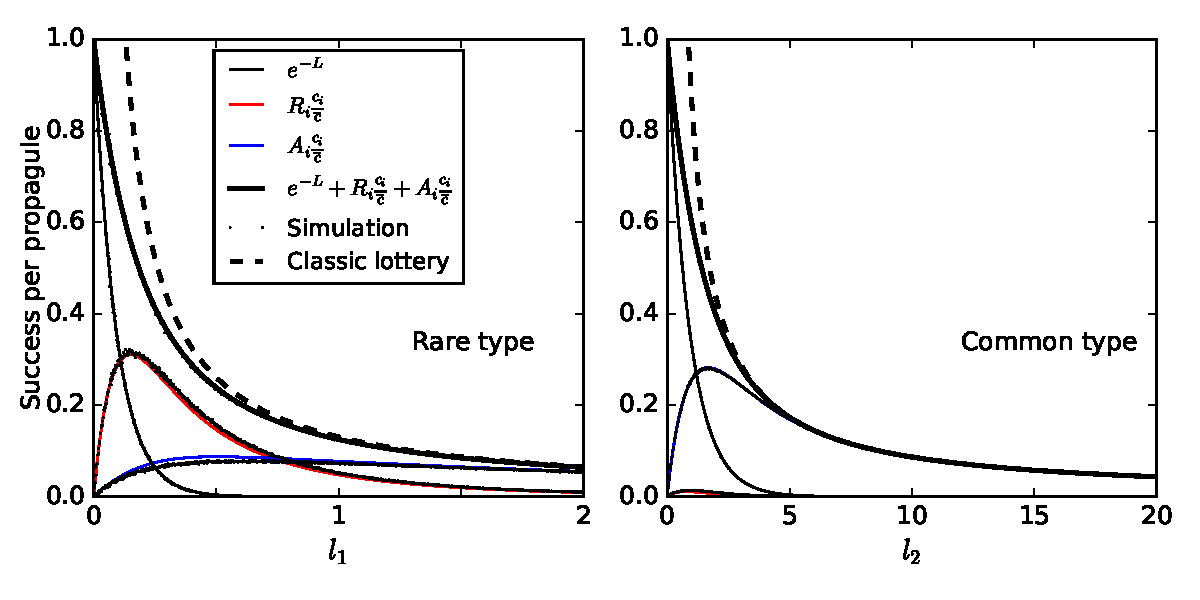
\includegraphics[scale=0.8]{simulationcomparison.pdf}
\caption{\label{fig:simcomp} Comparison of the analytical approximation Eq. \eqref{eq:master} with simulations. Per-propagule success probability $\Delta_+ n_i/l_i U$ from the classic lottery model, individual-based simulations of random dispersal and lottery competition, and Eq. \eqref{eq:master} and its three components. Two types are present, a rare type with $c_1=1.5$, and a common type with $c_2=1$. Simulation points are almost invisible in for the common type due to near exact agreement with Eq. \eqref{eq:master}. Dashed lines in show the breakdown of the classic lottery model. Parameters: $m_1=10^4$ and $m_2=9\times 10^4$ and $U$ varies between $5\times 10^3$ and $10^6$.} 
\end{figure}

Eq.~\eqref{eq:master} takes a much simpler form if all types are competitively equivalent ($c_i=c$),
\begin{equation}
\Delta_+ n_i = \frac{l_i}{L}(1-e^{-L})U. \label{eq:masterequalc}
\end{equation}
Here $1-e^{-L}$ is the fraction of territories that receive at least one propagule under Poisson dispersal, $(1-e^{-L})U$ is the total number of territories gained, and type $i$ receives a fraction $l_i/L$ of these. Total population density thus grows according to
\begin{equation}
\Delta N=(1-e^{-L})U-\sum_i d_i n_i \label{eq:Nmaster}
\end{equation}

\subsection*{Selection-dependent density and $K$-selection}

Equipped with our variable-density lottery model, we now start evaluating the validity of Eq.~\eqref{eq:canonical}. In this section we explore whether we should expect population density to vary as a result of selection \citep{prout_1980}. Since the idea that density does vary with selection is closely connected to the notion of ``$K$-selection'', we start by revisiting MacArthur's analysis of selection in crowded environments \citep{macarthur_1967}. 

MacArthur considers a population with two types that have densities $n_1$ and $n_2$ subject to density-dependent growth described by
\begin{equation}
\frac{d n_1}{d t}=f_1(n_1,n_2)\qquad\frac{d n_2}{d t}=f_2(n_1,n_2). \label{eq:macgeneral}
\end{equation}
The environment is assumed to remain constant apart from the type densities. The functions $f_1$ and $f_2$ must decline to zero if $n_1$ or $n_2$ are sufficiently large, because no population has unlimited resources. This defines the nullclines $f_1(n_1,n_2)=0$ and $f_2(n_1,n_2)=0$ in $(n_1,n_2)$ space. The outcome of selection is then determined by the relationship between these nullclines. Specifically, a type will be excluded if its nullcline is completely contained in the region bounded by the other type's nullcline. In other words, for a type to have the possibility of persisting, it must be able to keep growing to higher densities than the other type can tolerate in some region of $(n_1,n_2)$ space (Fig.~\ref{fig:Ksel}a).

To formalize the relationship between nullclines, MacArthur used the symbol ``$K$'' to label the four intersection points of the nullclines with the $n_1$ and $n_2$ axes, specifically $f_1(K_{11},0)=0$, $f_1(0,K_{12})=0$, $f_2(0,K_{22})=0$ and $f_2(K_{21},0)=0$. These $K$ values determine whether a region of higher-density growth exists for each type, provided that the nullclines are close to being straight lines. Note that only $K_{11}$ and $K_{22}$ are saturation densities akin to the $K$ parameter in the logistic model; following widespread convention, we will refer to selection on these saturation densities as ``$K$-selection'' (Fig.~\ref{fig:Ksel}a). The other intersection points, $K_{12}$ and $K_{21}$, are related to competition between types. For instance, in the Lotka-Volterra competition model we have
\begin{align}
f_1(n_1,n_2) = r_1(1-\alpha_{11}n_1-\alpha_{12}n_2)n_1\nonumber\\
f_2(n_1,n_2) = r_2(1-\alpha_{22}n_1-\alpha_{21}n_2)n_2\label{eq:LV}
\end{align}
where $\alpha_{11}=1/K_{11}$ and $\alpha_{22}=1/K_{22}$ measure competitive effects within types, while $\alpha_{12}=1/K_{12}$ and $\alpha_{21}=1/K_{21}$ measure competitive effects between types (Fig.~\ref{fig:LVvslottery}a). 

Thus, when MacArthur concludes that  ``fitness is $K$'' in crowded populations \citep[pp. 149]{macarthur_1967}, the meaning is that selection either favors the ability to keep growing at ever higher densities (moving a type's own nullcline outwards), or the ability to suppress the growth of competitors at lower densities (moving the nullcline of competitors inwards) \citep{gill_1974}. This general idea is much broader than ``$K$-selection'' in the sense of selection for greater saturation density, and applies even if the nullclines are nonlinear to such an extent that the ``$K$'' values themselves do not give much information about the regions of high-density growth.

\begin{figure}
\centering
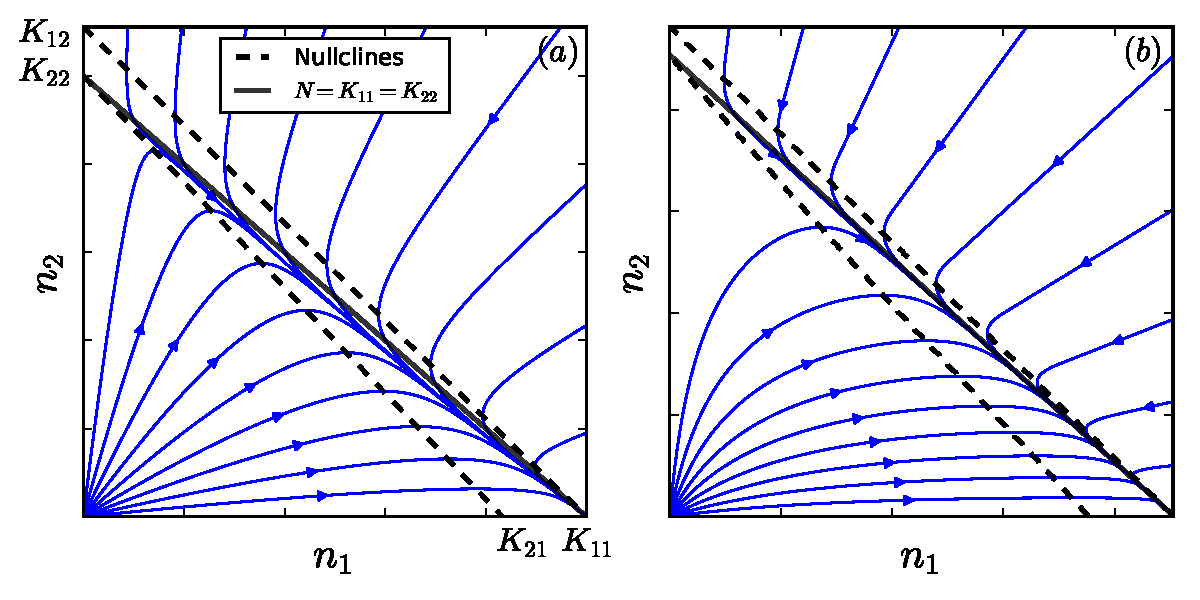
\includegraphics[scale=0.8]{LVvslottery.pdf}
\caption{\label{fig:LVvslottery} Selection between types with identical saturation density but different inter-type competitive ability. (a) Lotka-Volterra competition (Eq.~\ref{eq:LV}) with $r_1=r_2=1$, $\alpha_{11}=\alpha_{22}=1$, $\alpha_{12}=0.9$ and $\alpha_{21}=1.2$. Trajectories do not follow the line $N=K_{11}=K_{22}$. (b) Lottery competition (Eq.~\ref{eq:master}) with $b_1=b_2=5$, $d_1=d_2=0.1$ and $c_1/c_2=5$. Trajectories converge on the line $N=K_{11}=K_{22}$.}
\end{figure}

It is obvious from Eq.~\eqref{eq:LV} that selection can favor a superior competitor in a crowded population even if its saturation density is the same as, or lower than that of the other types present. However, the Lotka-Volterra model still couples selection to population density \citep{smouse_1976}. Fig.~\ref{fig:LVvslottery}a shows Lotka-Volterra selection between two types with the same saturation density ($\alpha_{11}=\alpha_{22}$, $\alpha_{21}>\alpha_{12}$). Even though the initial and final densities of a sweep are the same, density is not constant over a sweep. Only a highly restricted subset of $r$ and $\alpha$ values will keep $N$ constant over a selective sweep (further details in Appendix C). Intuitively, for one type to exclude another with the same saturation density, competitive suppression of growth between types must be stronger than competitive suppression of growth within types, causing a dip in $N$ over the sweep. 

By contrast, if one type in our density-dependent lottery model has a $c$ advantage but the types are otherwise identical (so that each type has the same saturation density), the density trajectories converge on the line of constant density equal to the saturation density (Fig.~\ref{fig:LVvslottery}b). Selection then occurs purely along this line, similarly to Fig.~\ref{fig:Ksel}b. This occurs because $c$ does not directly affect $N$: it only affects the relative likelihood for each type to win a contested territory, not whether a territory is contested in the first place (this can be seen formally in Eq.~\eqref{eq:Nmaster}). In other words, once the population reaches demographic equilibrium, it behaves indistinguishably from a constant-$N$ relative fitness model. While quite different from classical growth models like the Lotka-Volterra, this is all perfectly consistent with MacArthur's general argument. 

The constant-$N$ behavior of $c$-selection arises from the role of $c$ as a trait determining relative competitive success in territorial contests. As such, this behavior is a result of a reproductive excesses. By contrast, previous models of selection-independent density either used unusual models of competition \citep{kimura1969natural,nei1971fertility}, or made restrictive parameter choices in the Lotka-Volterra model (Appendix C; \citealt{smouse_1976,mallet_2012}). 

\subsection*{Density-regulating traits and the threat of strong selection}

In the previous section we showed that $c$-selection and the regulation of population density are independent even though population growth is density-regulated in our variable-density lottery. Nevertheless, selection and density regulation \textit{are} intimately connected in widely used models of population growth, as well as for the lottery $b$ and $d$ traits.

To see why this connection potentially poses a threat to relative fitness, consider the simple birth-death model \cite[pp. 20]{kostitzin_1939} \citep{travis_2013} 
\begin{equation}
\frac{d n_i}{dt}=(b_i -\delta_iN) n_i \label{eq:simplebirthdeath}
\end{equation}
where $\delta_i$ is the per-capita increase in mortality rate due to crowding (for simplicity, there are no deaths when uncrowded), playing a similar role as $K$ in the logistic model. 

Starting from a monomorphic population, the frequency of a $\delta_i\rightarrow \delta_i(1-\epsilon)$ variant obeys 
\begin{equation}
\frac{d p_i}{dt}=\epsilon \delta_i N p_i(1-p_i). \label{eq:Ndependentsweep}
\end{equation}
The selection coefficient $s=\epsilon \delta_i N$ thus depends on density (compare with Model III in \cite{kimura1969natural}). On the other hand, the frequency of a $b_i\rightarrow b_i(1+\epsilon)$ variant will exactly obey Eq.~\eqref{eq:canonical} with $s=\epsilon b_i$, independent of density.

In practice the density dependence in Eq.~\eqref{eq:Ndependentsweep} only matters if $N$ changes substantially during a sweep. This can easily occur if a population is far from demographic equilibrium (we return to this scenario in the Discussion). However, even if $N$ has reached equilibrium, it will change substantially over a $\delta$-sweep if selection on $\delta$ is sufficiently strong. To quantify this effect, we need to account for how much $N$ changes as a result of a $\delta$-sweep beginning and ending in equilibrium \citep{kimura1969natural}; from Eq.~\eqref{eq:simplebirthdeath} we have an increase from $N_{\rm initial}=b_i/\delta_i$ to $N_{\rm final}=b_i/\delta_i(1-\epsilon)=N_{\rm initial}/(1-\epsilon)$. The corresponding selection coefficient increases from $s_{\rm initial}= \epsilon b_i$ to $s_{\rm final}=s_{\rm initial}/(1-\epsilon)$. Consequently, noticeable deviations from Eq.~\eqref{eq:canonical} occur with proportional changes to $\delta$ of order $\epsilon=0.2$ and upwards i.e. selection must be quite strong (Fig.~\ref{fig:strengthofselection}). 

\begin{figure}
\centering
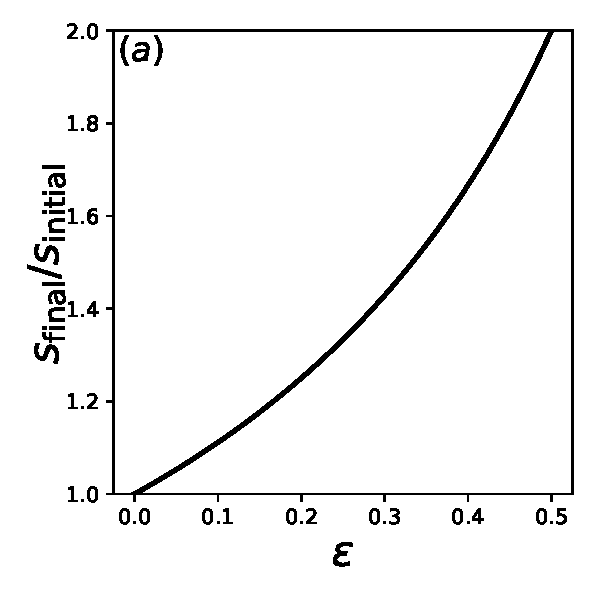
\includegraphics[scale=0.8]{strengthofselection.pdf}
\caption{\label{fig:strengthofselection} (a) Proportional change in the selection coefficient over a ``$K$-like'' sweep for a type that experiences proportionally $1-\epsilon$ fewer deaths induced by crowding. The population is in demographic equilibrium at the start and end of the sweep. (b) Example equilibrium-to-equilibrium $\delta$-sweep (Eq.~\ref{eq:Ndependentsweep}) for $\epsilon=0.2$ showing a noticeable deviation from the canonical selection equation.}
\end{figure}

Let us now turn to selection on $b$ and $d$ in our lottery model. Recall that $m_i=b_i n_i U/T$, and so $L=M/U=\overline{b}N/T$ where $\overline{b}$ is the population mean $b$. Thus, from Eq.~\eqref{eq:masterequalc} we have
\begin{equation}
\Delta n_i = \left(\frac{b_i}{\overline{b}}\frac{1-e^{-\overline{b}N/T}}{N}(T-N)-d_i\right)n_i. \label{eq:bdensitydependence}
\end{equation}
It can be seen that the mortality $d$ is akin to the birth rate in Eq.~\eqref{eq:simplebirthdeath}, and so, while $d$ does affect density, selection on $d$ is density independent. Thus, $d$ sweeps follow the canonical relative fitness model exactly (Fig.~\ref{fig:DDS_lottery}).

At first glance, $b$ in Eq.~\eqref{eq:bdensitydependence} appears to be analogous to the $\delta$ in Eq.~\eqref{eq:simplebirthdeath} because it regulates density and is multiplied by the density-dependent term $f(\overline{b},N)=\frac{1-e^{-\overline{b}N/T}}{N}(T-N)$. This term declines from $\overline{b}$ at low density to zero at high density and as a result, selection on $b$ is density-dependent. The source of this density-depedence is that the selective advantage from having greater $b$ depends on the number of territories being contested; if almost all are occupied, then there is little advantage to having a greater $b$.

Nevertheless, the behavior of equilibrium-to-equilibrium $b$-sweeps are qualitatively different from the $\delta$ sweeps above. The reason is that $b$ regulates density by controlling how many unoccupied territories receive propagules. Thus, greater $b$ means more propagules contesting territories, but also more territories being contested. The net effect on $f(\overline{b},N)$ is precisely zero in equilibrium: in a single-type equilibrium we have $b_i/\overline{b}=1$ and so $f(\overline{b},N)=d_i$ exactly at the beginning and end of a pure $b$ sweep, even though the density $N$ increases. Strictly speaking there is some deviation in $f(N)$ from $d_i$ during the sweep, but this deviation is an order of magnitude smaller than for a $\delta$ sweep (the deviation due to a sweep with proportional effect $b_i\rightarrow b_i(1+\epsilon)$ is only of order $\epsilon^2$, whereas the analogous effect in Fig.~\ref{fig:strengthofselection} is of order $\epsilon$; see Appendix D for details). Since selection must already be quite strong for a $\delta$ sweep to threaten Eq.~\eqref{eq:canonical}, we conclude that $b$ sweeps also obey the canonical selection equation (to a close approximation). 

\begin{figure}
\centering
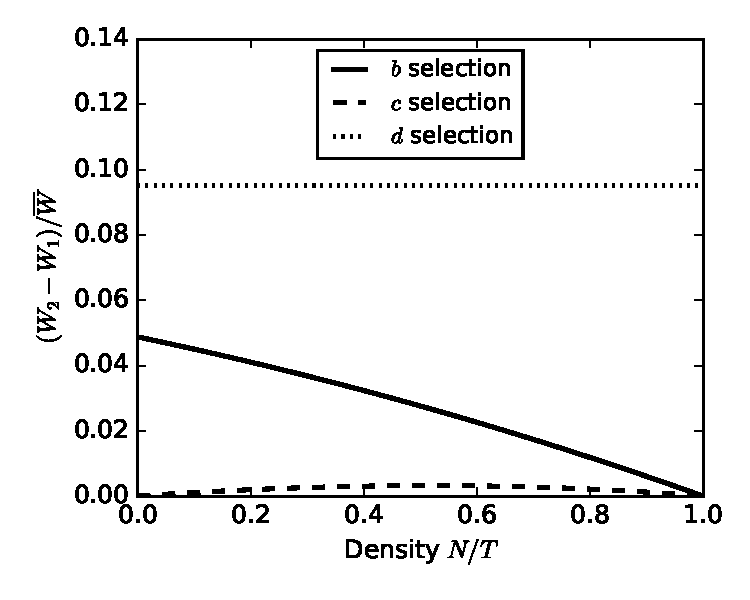
\includegraphics[scale=0.8]{DDS_lottery.pdf}
\caption{\label{fig:DDS_lottery} The density-dependence of selection in our variable-density lottery plotted as the selection coefficient $(\Delta n_j-\Delta n_i)/n_j$ experienced by an adaptive variant $j$ present at the same frequency as a wildtype $i$. Here $b_i=1$, $d_i=0.5$ and $c_i=1$. For $b$-selection we set $b_j=b_i(1+\epsilon)$, and similarly for $c$ and $d$, with $\epsilon=0.1$. $d$-selection is density-independent, $b$-selection gets weaker with lower territorial availability, while $c$-selection initially increases with density as territorial contests become more important, but eventually also declines as  available territories become scarce. The equilibrium density for the $i$ type is $\approx 0.4$.}
\end{figure}

\section*{Discussion}

Summarizing the three traits in the variable-density lottery model: (i) $c$-selection is density-dependent, but $c$ does not regulate density; (ii) $d$ regulates density, but $d$-selection is density-independent; (iii) $b$ regulates density and $b$-selection is density-dependent. Despite these differences, pure $b$, $c$ and $d$ sweeps starting and ending at equilibrium all obey the canonical selection equation. This rich variety of behaviors in relation to density is quite different from that found in the classical density-dependent selection literature \citep{roughgarden_1979,christiansen_2004}. 

To briefly review: based on a diploid, bi-allelic variant of the logistic model, the $r$/$K$ scheme proposed a dichotomy between $r$-selection (uncrowded) and $K$-selection (crowded) \citep{macarthur_1962}, with the latter taken to mean selection for greater saturation density \citep{gill_1974}. A more general Lotka-Volterra model introduces the inter-type $\alpha_{ij}$ competition coefficients, with selection on these termed ``$\alpha$-selection'' \citep{gill_1974,joshi_2001}. Setting aside $r$ which confers no selective advantage at equilibrium, we are left with $K$ and $\alpha$, which both behave like $\delta$ in that they are density-dependent and cause density to change over a sweep (although $N$ only dips temporarily during an $\alpha$-sweep). Thus, strong selection is sufficient for relative fitness to break down in the classical view of density-dependent selection. Indeed, in the defense of Eq.~\eqref{eq:canonical} given by \cite{kimura1969natural}, it was assumed that $s$ will be a few percent at most. While this may be reasonable for adaptive mutations, there is no reason to expect selection on standing variation to be so weak, wild \textit{Drosophila} being an obvious counter-example \citep{bergland_14}.

Our variable-density lottery model shows that it is not simply a lack of ecological realism that underlies the contrast between relative fitness and the classical view of density-dependent selection. Rather, in many population growth models, only one life-history stage is represented, and the competitive effects resulting from crowding appear as a reduction in absolute fitness that only depends on the type densities at this life-history stage (e.g. the $n_i^2$ and $n_in_j$ terms in the Lotka Volterra equation). As noted in the introduction, this precludes selection concentrated at a fragile juvenile stage as a result of a reproductive excess \citep{chesson_1983,turner1968population,kimura1969natural,nei1971fertility}. 

Reproductive excesses appear in the variable-density lottery model when the number of propagules is greater than the number of available territories. Then only $\approx 1/L$ of the juveniles contesting available territories survive to adulthood. Unlike the role of adult density $n_i$ in single-life-stage models, it is the propagule densities $l_i$ that represent the crowding that drives competition (a ``critical age-group''; \citealt[pp. 54]{charlesworth_1994}). In general, reproductive excesses will tend to produce strictly-relative lottery-type contests in which fitter types grow at the expense of others by preferentially filling the available adult ``slots''. The number of slots can remain fixed or change independently of selection at the juvenile stage. By ignoring reproductive excesses, single life-stage models are biased to have total population density be sensitive to ongoing selection. In this respect, the Wright-Fisher model and similar viability selection heuristics actually capture an important ecological process.

We now turn to the breakdown of Eq.~\eqref{eq:canonical}. We first discuss the problem shown in Fig.~\ref{fig:strengthofselection}, which occurs when strong selection changes population density and is also density-dependent. In the variable-density lottery, this occurs if and only if types differ in more than one trait. The $c$ and $d$ traits represent the two distinct directions in which density and selection interact: selection may depend on density, and density may depend on selection \citep{prout_1980}. The combination is necessary to pose a threat to Eq.~\eqref{eq:canonical}. However, the $b$ trait remarkably demonstrates that the combination is not sufficient, since the density-dependence of $b$-selection disappears over equilibrium-to-equilibrium $b$-sweeps. Thus, the simple linear models that have become standard in discussions of density-dependent selection \citep{roughgarden_1979,christiansen_2004,mallet_2012,travis_2013} actually represent a complicated form of the interaction between density and selection, and their parameters confound the underlying issues. 

While this is a conceptual reason to be wary of the classical density-dependent selection models, it is not clear how we should expect the trait variation in nature to align. For instance, should we expect mutations to generally affect $b$, $c$ and $d$ independently of each other, or pleiotropically such that $\delta$-like selection is prevalent? In the case of well-mixed indirect exploitation competition for consumable resources, the $R^*$ rule  suggests that $\delta$-like selection will be prevalent. However, for many populations consumable resources are not well-mixed. Spatial localization of consumable resources (e.g. due to restricted movement of  nutrients through soils) will tend to create a territorial situation similar to the lottery model, where resource competition only occurs locally and both it any interference competition are subsumed into the competitive ability $c$, which does not affect $N$. 

Relative fitness models truly break down when $N$ is far from equilibrium and selection is density-dependent (as seems likely; \citealt{travis_2013}). For example, wild \textit{Drosophila} experience large seasonal boom-bust cycles in population density coupled to strong selection that drives large swings in allele frequency \citep{bergland_14}. In this case there is no choice but to abandon relative fitness, and our model provides one potentially suitable option. Whether or not our density-dependent lottery model is a good description of \textit{Drosophila} ecology, the close connection between our model and Wright-Fisher is useful, because drift in our model should behave broadly similarly. Thus, our model it should provide a useful starting point for analyzing evolution in this and other far-from-equilibrium situations. 

Another issue with the constant-$N$ relative fitness description of selection is that it precludes consideration of longer-term aspects of the interplay between evolution and ecology such as population extinction. A variety of approaches have been developed for dealing with these issues in quantitative genetics \citep{burger1995evolution,engen_2013}, population genetics \citep{bertram2017predicting} and adaptive dynamics \citep{ferriere2013eco,dieckmann2004adaptive}. Although density-dependent selection is  pertinent to these longer-term issues \citep{travis_2013}, our focus here has been the description of the time-dependent process by which selection changes allele frequencies. This is particularly critical for making sense of evolution at the genetic level, for which we now have abundant data.


\bibliographystyle{abbrvnat}
\bibliography{reference} 

\section*{Appendix A: Poisson dispersal}

For simplicity of presentation, we assume a Poisson distribution for the $x_i$ as our model of dispersal. Strictly speaking, the total number of $i$ propagules $\sum x_i$ (summed over unoccupied territories) is then no longer a constant $m_i$, but fluctuates between generations for a given mean $m_i$. Nevertheless, since we do not consider the random fluctuations in type abundances here, and for ease of comparison with the classic lottery model, we ignore the fluctuations in $m_i$. Instead we focus on Poisson fluctuations in propagule composition in each territory. 

In the exact model of random dispersal, the counts of a type's propagules across unnocupied territories follows a multinomial distribution with dimension $U$, total number of trials equal to $m_i$, and equal probabilities $1/U$ for a propagule to land in a given territory. Thus, the $x_i$ in different territories are not independent random variables. However, for sufficiently large $U$ and $m_i$, this multinomial distribution for the $x_i$ across territories is closely approximated by a product of independent Poisson distributions for each territory, each with rate parameter $l_i$ \citep[Theorem 1]{arenbaev_1977}. Since we are ignoring finite population size effects, we effectively have $T\rightarrow \infty$, in which case $U$ can only be small enough to violate the Poisson approximation if there is vanishing population turnover, and then the dispersal distribution is irrelevant anyway. Likewise, in ignoring stochastic finite population size for the $n_i$, we have effectively already assumed that $m_i$ is large enough to justify the Poisson approximation (the error scales as $1/\sqrt{m_i}$; \citealt{arenbaev_1977}).

\section*{Appendix B: Growth equation derivation}

In this appendix we derive Eq.~\eqref{eq:master}. We start by separating the right hand side of Eq.~\eqref{eq:growthsumuncoupled} into three components
\begin{equation}
\Delta_+ n_i = \Delta_u n_i+\Delta_r n_i+\Delta_a n_i,
\end{equation}
which vary in relative magnitude depending on the propagule densities $l_i$. The first component, $\Delta_u n_i$, accounts for territories where only one focal propagule is present ($x_i=1$ and $x_j=0$ for $j\neq i$; $u$ stands for ``uncontested''). The proportion of territories where this occurs is $l_i e^{-L}$, and so 
\begin{equation}
\Delta_u n_i=Ul_i e^{-L}=m_i e^{-L}.
\end{equation}

The second component, $\Delta_r n_i$, accounts for territories where a single focal propagule is present along with at least one non-focal propagule ($x_i=1$ and $X_i\geq 1$ where $X_i=\sum_{j\neq i} x_j$ is the number of nonfocal propagules; $r$ stands for ``rare''). The number of territories where this occurs is $Up_i(1)P(X_i\geq 1)=m_i e^{-l_i}(1-e^{-(L-l_i)})$. Thus 
\begin{equation}
\Delta_r n_i = m_i e^{-l_i}(1-e^{-(L-l_i)})\left\langle  \frac{c_i}{c_i +\sum_{j\neq i} c_j x_j } \right\rangle_{\tilde{p}},  \label{eq:deltr}
\end{equation}
where $\langle \rangle_{\tilde{p}}$ denotes the expectation with respect to the probability distribution $\tilde{p}$ of nonfocal propagule abundances $x_j$, in those territories where exactly one focal propagule, and at least one non-focal propagule, landed. 

The final contribution, $\Delta_a n_i$, accounts for territories where two or more focal propagules are present ($x_i\geq 2$; $a$ stands for ``abundant"). Similar to Eq.~\eqref{eq:deltr}, we have 
\begin{equation}
\Delta_a n_i=U(1-(1+l_i)e^{-l_i})\left\langle \frac{c_i x_i}{\sum_j c_j x_j} \right\rangle_{\hat{p}}\label{eq:delta}
\end{equation}
where $\hat{p}$ is the probability distribution of both focal and nonfocal propagule abundances in those territories where at least two focal propagules landed. 

To derive Eq.~\eqref{eq:master} we approximate the expectations in Eq.~\eqref{eq:deltr} and Eq.~\eqref{eq:delta} by replacing $x_i$ and the $x_j$ with ``effective'' mean values as follows 
\begin{equation}
\left\langle\frac{c_i}{c_i +\sum_{j\neq i} c_j x_j}\right\rangle_{\tilde{p}}\approx \frac{c_i}{c_i +\sum_{j\neq i} c_j \langle x_j\rangle_{\tilde{q}}}.\label{eq:meanfieldr}
\end{equation}
\begin{equation}
\left\langle \frac{c_i x_i}{\sum_j c_j x_j} \right\rangle_{\hat{p}}\approx  \frac{c_i \langle x_i \rangle_{\hat{q}}}{\sum_j c_j \langle x_j\rangle_{\hat{q}}}.\label{eq:meanfielda}
\end{equation}
Here the effective means $\langle \rangle_{\tilde{q}}$ and $\langle \rangle_{\hat{q}}$ are taken with respect to new distributions $\tilde{q}$ and $\hat{q}$, respectively. In the following subsection we define $\tilde{q}$ and $\hat{q}$ and explain our reasoning for using these distributions to take the effective means. 

\subsection*{The effective distributions $\tilde{q}$ and $\hat{q}$}

The approximations \eqref{eq:meanfieldr} and \eqref{eq:meanfielda} must be done in a way that ensures consistency between rare and common types. To illustrate, suppose that two identical types are present (same $b$, $c$ and $d$), one with low density $l_1\ll 1$, and the other with high density $l_2\approx L\gg 1$. Since $L$ is large, uncontested territories contribute negligibly to each type's growth. The rare type grows almost entirely due to $\Delta_r n_1$, while the common type grows almost entirely due to $\Delta_a n_2$. To ensure consistency, the approximate per-capita growth rates $\Delta_r n_1/m_1 = \Delta_a n_2/m_2$ implied by \eqref{eq:meanfieldr} and \eqref{eq:meanfielda} must be equal. Even small violations of this consistency condition will cause one type to grow exponentially relative to the other. This is a logical contradiction: any single-type population can be divided at will into rare and common subsets of identical types, and clearly not all such subsets can grow/decline.

For example, suppose that we use $\tilde{p}$ and $\hat{p}$ in place of $\tilde{q}$ and $\hat{q}$ in Eqs.~\eqref{eq:meanfieldr} and \eqref{eq:meanfielda}, respectively. Then, since $\langle x_2\rangle_{\tilde{p}}\approx L$, the right hand side of Eq. \eqref{eq:meanfieldr} is approximately $1/(L+1)$ for the rare type. And, since $l_1\ll 1$ and $L\gg 1$ in Eq.~\eqref{eq:deltr}, we have $\Delta_r n_1 \approx 1/(L+1)$. Similarly, for the common type, $\sum_j \langle x_j\rangle_{\hat{p}}\approx L$ in Eq. \eqref{eq:meanfielda}, and so $\Delta_a n_2 \approx 1/L$. Therefore, the consistency requirement is violated if we naively use the conditional distributions $\tilde{p}$ and $\hat{p}$ derived from the dispersal distribution $p$ to calculate the effective means. 

The effective distributions $\tilde{q}$ and $\hat{q}$ are chosen to ensure that this consistency requirement is satisfied. 

$\tilde{p}$ assumes that one of the propagules present in a given territory after dispersal belongs to the focal type (a statement about propagule identity), whereas $\tilde{q}$ assumes that there is a focal propagule present before non-focal dispersal commences (a statement about propagule presence). 


%Following the notation in the main text, the Poisson distributions for the $x_i$ (or some subset of the $x_i$) will be denoted $p$, and we use $P$ as a general shorthand for the probability of particular outcomes.

By contrast, Eq. \eqref{eq:meanxjrare} correctly predicts that there are on average $\sum_{j\neq i}\langle x_j \rangle_{\tilde{p}}\approx L-1$ nonfocal propagules because $\tilde{p}$ accounts for potentially large negative covariances between the $x_j$ ``after dispersal''. By neglecting the latter covariances, $\tilde{q}$ overestimates the fluctuations in $\sum_{j\neq i} c_j x_j$; thus $\tilde{q}$ gives an upper bound on the fluctuations. The discrepancy between $\tilde{q}$ and $\tilde{p}$ will be largest when $L$ is of order $1$ or smaller, because then the propagule assumed to already be present under $\tilde{q}$ is comparable to, or greater than, the entire propagule density.






Below we justify this replacement by arguing that the standard deviation $\sigma_{\tilde{p}}(\sum_{j\neq i} c_j x_j)$ (with respect to $\tilde{p}$), is much smaller than $\langle\sum_{j\neq i} c_j x_j\rangle_{\tilde{p}}$. If this standard deviation is small as claimed, then the mean value gives an accurate representation of the values taken by $\sum_{j\neq i} c_j x_j$ across territories. 

We first calculate $\langle x_j \rangle_{\tilde{p}}$. Let $X=\sum_j x_j$ denote the total number of propagules in a territory and ${\mathbf x_i}=(x_1,\ldots,x_{i-1},x_{i+1}\ldots,x_G)$ denote the vector of non-focal abundances, so that $p({\mathbf x_i})=p_1(x_1)\cdots p_{i-1}(x_{i-1})p_{i+1}(x_{i+1})\cdots p_G(x_G)$. Then, $\tilde{p}$ is the probability distribution for ${\mathbf x_i}$ conditional on the territory having received $X\geq 2$ propagules, where $X_i=X-1$ of them are nonfocal, giving
\begin{equation}
\tilde{p}({\mathbf x_i})=\sum_{X=2}^{\infty}P(X|X\geq 2) p({\mathbf x_i}|X_i=X-1)
\end{equation}
Here the total number of propagules $X$ follows a Poisson distribution with mean $L$, and we have $P(X|X\geq 2)=P(X)/P(X\geq 2)=P(X)/(1-(1+L)e^{-L})$. Thus,
\begin{align}
\langle x_j \rangle_{\tilde{p}}&=\sum_{\mathbf x_i} \tilde{p}({\mathbf x_i})x_j\nonumber\\
&=\frac{1}{1-(1+L)e^{-L}}\sum_{X=2}^{\infty} P(X) \sum_{\mathbf x_i} p({\mathbf x_i}|X_i=X-1)x_j.
\label{eq:raremonster1}
\end{align}
The inner sum over ${\mathbf x_i}$ is the mean number of propagules of a given nonfocal type $j$ that will be found in a territory which received $X-1$ nonfocal propagules in total, which is equal to $\frac{l_j}{L-l_i}(X-1)$. Thus, 
\begin{align}
\langle x_j \rangle_{\tilde{p}}&=\frac{l_j}{1-(1+L)e^{-L}}\frac{1}{L-l_i}\sum_{X=2}^{\infty} P(X) (X-1)\nonumber\\
&=\frac{l_j}{1-(1+L)e^{-L}}\frac{L-1+e^{-L}}{L-l_i},
\label{eq:meanxjrare}
\end{align}
where the last line follows from $\sum_{X=2}^{\infty} P(X)(X-1)=\sum_{X=1}^{\infty} P(X)(X-1)=\sum_{X=1}^{\infty} P(X)X-\sum_{X=1}^{\infty}P(X)$.

Having evaluated the mean propagule numbers, we now evaluate the variance in propagule numbers to check that the mean value replacement in Eq.~\eqref{eq:meanfieldr} is justified. This is complicated because the $x_j$ are not independent with respect to $\tilde{p}$. Here we use the following approximation to give some insight into the magnitude of these fluctuations and also the nature of the correlations between the $x_j$. We replace $\tilde{p}$ with $\tilde{q}$, defined as the ${\mathbf x_i}$ Poisson dispersal probabilities conditional on $X_i\geq1$ (which are independent). The distinction between $\tilde{p}$ and $\tilde{q}$ will be discussed further below. The $\tilde{q}$ approximation gives $\langle x_j \rangle_{\tilde{q}}=\langle x_j \rangle_p/C=l_j/C$, where $C=1-e^{-(L-l_i)}$, with variances and covariances given by
\begin{align}
\sigma_{\tilde{q}}^2(x_j)&=\langle x_j^2 \rangle_{\tilde{q}}-\langle x_j \rangle_{\tilde{q}}^2\nonumber\\
&=\frac{1}{C}\langle x_j^2 \rangle_p-\frac{l_j^2}{C^2}\nonumber \\
&=\frac{1}{C}(l_j^2 + l_j)-\frac{l_j^2}{C^2}\nonumber \\
&=\frac{l_j^2}{C}\left(1-\frac{1}{C}\right)+\frac{l_j}{C},\label{eq:varr}
\end{align}
and 
\begin{align}
\sigma_{\tilde{q}}(x_j,x_k)&=\langle x_j x_k \rangle_{\tilde{q}}-\langle x_j \rangle_{\tilde{q}}\langle x_k \rangle_{\tilde{q}}\nonumber\\
&=\frac{1}{C}\langle x_j x_k \rangle_p-\frac{l_jl_k}{C^2}\nonumber\\
&=\frac{l_j l_k}{C}\left(1-\frac{1}{C}\right)\qquad\qquad j\neq k. \label{eq:covr}
\end{align} 

Decomposing the variance in $\sum_{j\neq i} c_j x_j$,
\begin{equation}
\sigma_{\tilde{q}}^2(\sum_{j\neq i} c_j x_j)=\sum_{j\neq i}\left[c_j^2\sigma_{\tilde{q}}^2(x_j)+2\sum_{k>j, k\neq i}c_j c_k\sigma_{\tilde{q}}(x_j,x_k)\right],\label{eq:vartotr}
\end{equation}
and using the fact that $\sigma_{\tilde{q}}(x_j,x_k)$ and the first term in Eq. \eqref{eq:varr} are negative because $C<1$, we obtain an upper bound on the relative fluctuations in $\sum_{j\neq i} c_j x_j$, 
\begin{equation}
\frac{\sigma(\sum_{j\neq i} c_j x_j)}{\langle\sum_{j\neq i} c_j x_j\rangle}=C^{1/2}\frac{\left(\sum_{j\neq i}c_j^2 l_j+(1-1/C)\left(\sum_{j\neq i}c_j l_j\right)^2 \right)^{1/2}}{\sum_{j\neq i}c_j l_j}<C^{1/2}\frac{\left(\sum_{j\neq i}c_j^2 l_j\right)^{1/2}}{\sum_{j\neq i}c_j l_j}. \label{eq:cvr}
\end{equation}

Suppose that the $c_j$ are all of similar magnitude (their ratios are of order one). Then Eq.~\eqref{eq:cvr} is $\ll 1$ for the case when $L-l_i \ll 1$ (due to the factor of $C^{1/2}$), and also for the case when at least some of the nonfocal propagule densities are large $l_j\gg 1$ (since it is then of order $1/\sqrt{L-l_i}$). The worst case scenario occurs when $L-l_i$ is of order one. Then Eq.~\eqref{eq:cvr} gives a relative error of approximately $50\%$, which from our earlier discussion we know to be a substantial overestimate when $L$ is of order $1$. Our numerical results (Fig. \ref{fig:simcomp}) confirm that the relative errors are indeed small.

However, the relative fluctuations in $\sum_{j\neq i} c_j x_j$ can be large if some of the $c_j$ are much larger than the others. Specifically, in the presence of a rare, extremely strong competitor ($c_j l_j\gg c_{j'} l_{j'}$ for all other nonfocal types $j'$, and $l_j\ll 1$), then the RHS of Eq. \eqref{eq:cvr} can be large and we cannot make the replacement Eq.~\eqref{eq:meanfieldr}. 

Substituting Eqs. \eqref{eq:meanfieldr} and \eqref{eq:meanxjrare} into Eq.~\eqref{eq:deltr}, we obtain
\begin{equation}
\Delta_r n_i\approx m_i R_i\frac{c_i}{\overline{c}}, \label{eq:deltrfinal}
\end{equation}
where $R_i$ is defined in Eq.~\eqref{eq:Dr}.

\subsection*{Competition when abundant}



Again, we argue that the relative fluctuations in $\sum c_j x_j$ are much smaller than $1$ (with respect to $\hat{p}$), so that,


Following a similar procedure as for $\Delta_r n_i$, where the vector of propagule abundances is denoted ${\mathbf x}$, the mean focal type abundance is, 
\begin{align}
\langle x_i \rangle_{\hat{p}}&=\sum_{\mathbf x} x_i p(\mathbf x|x_i\geq 2)\nonumber \\
&=\sum_{x_i} x_i p(x_i|x_i\geq 2) \nonumber\\
&=\frac{1}{1-(1+l_i)e^{-l_i}}\sum_{x_i\geq 2} p(x_i)x_i\nonumber\\
&=l_i\frac{1-e^{-l_i}}{1-(1+l_i)e^{-l_i}}.
\end{align}
For nonfocal types $j\neq i$, we have
\begin{align}
\langle x_j \rangle_{\hat{p}}&=\sum_{\mathbf x} x_j p(\mathbf x|x_i\geq 2)\nonumber \\
&=\sum_{X}P(X|x_i\geq 2)\sum_{\mathbf x} x_j p({\mathbf x}|x_i\geq 2,X)\nonumber\\
&=\sum_{X}P(X|x_i\geq 2)\sum_{x_i} p(x_i|x_i\geq 2,X) \sum_{\mathbf x_i} x_j p(\mathbf x_i|X_i=X-x_i)\nonumber\\
&=\sum_{X}P(X|x_i\geq 2)\sum_{x_i}p(x_i|x_i\geq 2,X) \frac{l_j(X-x_i)}{L-l_i} \nonumber\\
&=\frac{l_j}{L-l_i}\left[\sum_{X}P(X|x_i\geq 2)X - \sum_{x_i}p(x_i|x_i\geq 2) x_i \right]\nonumber\\
&=\frac{l_j}{L-l_i}\left( L\frac{1-e^{-L}}{1-(1+L)e^{-L}}- l_i\frac{1-e^{-l_i}}{1-(1+l_i)e^{-l_i}}\right).
\end{align}
In going from line 3 to 4, we used the same logic used to evaluate the inner sum in Eq.~\eqref{eq:raremonster1}, and in going from 4 to 5 we have separately evaluated the contributions from the $X$ and $x_i$ terms in the numerator.

To calculate the standard deviation in $\sum_{j\neq i} c_j x_j$, we use a similar approximation as for $\Delta_r n_i$: $\hat{p}$ is approximated by $\hat{q}$, defined as the ${\mathbf x}$ dispersal probabilities in a territory conditional on $x_i>2$ (that is, treating the $x_j$ as independent). All covariances between nonfocal types are now zero, so that $\sigma_{\hat{q}}^2(\sum c_j x_j)=\sum c_j^2 \sigma_{\hat{q}}^2(x_j)$, where $\sigma_{\hat{q}}^2(x_j)=l_j$ for $j\neq i$, and  
\begin{equation}
\sigma_{\hat{q}}^2(x_i)=\frac{l_i}{D}\left(l_i+1-e^{-l_i}-\frac{l_i}{D}\left(1-e^{-l_i}\right)^2\right),
\end{equation}
where $D= 1-(1+l_i)e^{-l_i}$, and 
\begin{equation}
\frac{\sigma_{\hat{q}}(\sum c_j x_j)}{\langle\sum c_j x_j\rangle} = \frac{\left(\sum_{j\neq i} c_j^2 l_j + c_i^2 \sigma_{\hat{q}}^2(x_i)\right)^{1/2}}{\sum_{j\neq i} c_j l_j + c_i l_i (1-e^{-l_i})/D} \label{eq:cva}.
\end{equation}

Similarly to Eq.~\eqref{eq:cvr}, the RHS of Eq. \eqref{eq:cva} is $\ll 1$ for the case that $L \ll 1$ (due to a factor of $D^{1/2}$), and also for the case when at least some of the propagule densities (focal or nonfocal) are large --- provided that $c_i$ and the $c_j$ are all of similar magnitude. Again, the worst case scenario occurs when $l_i$ and $L-l_i$ are of order $1$, in which case Eq. \eqref{eq:cva} is around $35\%$, which is again where the $\hat{q}$ approximation produces the biggest overestimate of the fluctuations in ${\mathbf x}$. Similarly to Eq.~\eqref{eq:cvr}, the RHS of \eqref{eq:cva} will not be $\ll 1$ in the presence of a rare, extremely strong competitor.  

Combining Eqs. \eqref{eq:delta} and \eqref{eq:meanfielda}, we obtain
\begin{equation}
\Delta_a n_i=m_i A_i \frac{c_i}{\overline{c}},
\end{equation}
where $A_i$ is defined in Eq.~\eqref{eq:Da}.

\section*{Appendix C: Total density in the Lotka-Volterra competition model}

Here we show that under the Lotka-Volterra model of competition, total density $N$ does not in general remain constant over a selective sweep in a crowded population even if the types have the same saturation density (for a related discussion on the density- and frequency-dependence of selection in the Lotka-Volterra model, see \citep{smouse_1976,mallet_2012}).

We assume equal effects of crowding within types $\alpha_{11}=\alpha_{22}=\alpha_{\rm intra}$ and $N=1/\alpha_{\rm intra}$ and check whether it is then possible for $\frac{dN}{dt}$ to be zero in the sweep ($n_1,n_2 \neq 0$). Substituting these conditions into Eq.~\eqref{eq:LV}, we obtain 
\begin{align}
\frac{d n_1}{dt} = r_1(\alpha_{11}-\alpha_{12})n_1n_2 \nonumber\\
\frac{d n_2}{dt} = r_2(\alpha_{22}-\alpha_{21})n_1n_2
\end{align}
Adding these together, $\frac{dN}{dt}$ can only be zero if 
\begin{equation}
r_1(\alpha_{\rm intra}-\alpha_{12})+r_2(\alpha_{\rm intra}-\alpha_{21})=0. \label{eq:constNcondition}
\end{equation}
To get some intuition for Eq.~\eqref{eq:constNcondition}, suppose that a mutant arises with improved competitive ability but identical intrinsic growth rate and saturation density ($r_1=r_2$ and $\alpha_{11}=\alpha_{22}$). This could represent a mutation to an interference competition trait, for example \citep{gill_1974}. Then, according the above condition, for $N$ to remain constant over the sweep, the mutant must find the wildtype more tolerable than itself by exactly the same amount that the wildtype finds the mutant less tolerable than itself. 

Even if we persuaded ourselves that this balance of inter-type interactions is plausible in some circumstances, when multiple types are present the requirement for constant $N$ becomes
\begin{equation}
\sum_{ij}r_i(\alpha_{\rm intra}-\alpha_{ij})p_ip_j=0,
\end{equation}
which depends on frequency and thus cannot be satisfied in general for constant inter-type coefficients $\alpha_{ij}$. We conclude that selection in the Lotka-Volterra competition model will generally involve non-constant $N$.

\section*{Appendix D: Density-dependence of $b$-selection}

In section ``Density-regulating traits and the threat of strong selection'' we argued that the density-dependent factor $f(\overline{b},N)$ is unchanged at the beginning and end points of an equilibrium-to-equilibrium $b$. Here we estimate the magnitude of the deviation in $f(\overline{b},N)$ during the sweep. 

For simplicity, we introduce the notation $D=N/T$ and assume that $D$ is small. We can thus make the approximation $1-e^{-\overline{b}D}\approx \overline{b}D$ and $f(\overline{b},N)\approx \overline{b}(1-D)$. We expect this to be a conservative approximate based on the worst case scenario, because $N$ is most sensitive to an increase in $b$ in this low-density linear regime. We first calculate the value of $f(\overline{b},N)$ at the halfway point in a sweep, where the halfway point is estimated with simple linear averages for $b$ and $N$. The sweep is driven by a $b$ variant with $b_j=b_i(1+\epsilon)$, and we denote the corresponding initial and final densities by $D_i$ and $D_j$ respectively, where we have $d_i=b_i(1-D_i)=b_j(1-D_j)$. We obtain
\begin{align}
f_{\rm{half}}=f(\frac{b_i+b_j}{2},\frac{N_i+N_j}{2})&=\frac{b_i+b_j}{2}\left(1-\frac{D_i+D_j}{2}\right) \nonumber \\
&=\frac{1}{4} (b_i+b_j)(2-D_i-D_j) \nonumber \\
&=\frac{1}{4} (2d_i+b_i(1-D_j)+b_j(1-N_i)).
\end{align}
Dividing by $d_i$, the proportional deviation in $f(N)$ at the midpoint of the sweep is
\begin{align}
\frac{f_{\rm{half}}}{d_i}&=\frac{1}{4}\left(2+\frac{b_i}{b_j}+\frac{b_j}{b_i}\right)\nonumber \\
&=\frac{1}{4}\left(2+\frac{1}{1+\epsilon}+1+\epsilon\right)\nonumber \\
&=1+\frac{1}{4}(\epsilon^2-\epsilon^3+\ldots),
\end{align}
where we have used the Taylor expansion $\frac{1}{1+\epsilon}=1-\epsilon+\epsilon^2-\epsilon^3+\ldots$. 

By contrast, for a $\delta$ sweep in Eq.~\eqref{eq:simplebirthdeath}, the density-dependent term $N$ increases by a factor of $\frac{1}{1-\epsilon}=1+\epsilon+\epsilon^2+\ldots$. Thus,  the deviations in $f(N)$ are an order of magnitude smaller than those shown in Fig.~\eqref{fig:strengthofselection}, and even proportional changes of order $\epsilon=0.1$ will cause a negligible deviation from the canonical selection equation.


\end{document}

